\documentclass[10pt,a4paper]{beamer}
\usepackage[utf8]{inputenc}
\usepackage[english]{babel}
\usepackage[T1]{fontenc}
\usepackage{amsmath}
\usepackage{amsfonts}
\usepackage{amssymb}
\usepackage{graphicx}

\usetheme{Warsaw}
\usecolortheme{beaver}
\usecolortheme{orchid}
\author{Ludovic}
\begin{document}
\section{Introduction}
\subsection{Les bases}

% SLIDE INTRODUCTION
\begin{frame}{Introduction}
  \begin{block}{Des choses}
    \begin{itemize}
    \item Une chose,
    \pause
    \item Une autre chose
    \end{itemize}
  \end{block}
\end{frame}

\subsection{Les volatiles marins}


\begin{frame}{La glisse du pingouin}
  \begin{columns}[c]
      \column{.5\textwidth}
        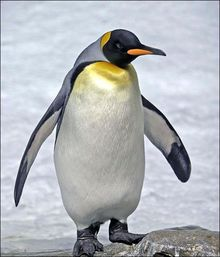
\includegraphics[width = \textwidth]{pingouin.jpg}<1>
        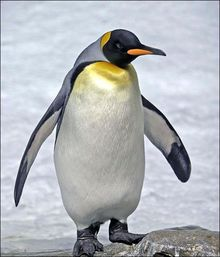
\includegraphics[angle = 180, width = \textwidth]{pingouin.jpg}<2->
      \column{.5\textwidth}
        \begin{block}{La glisse}
          \begin{itemize}
          \item<1-3> Il glisse toujours,          
          \item<2> Parfois sur la glace,          
          \item<3> Ou sur la route.
          \end{itemize}
       \end{block}
  \end{columns}
  \transdissolve
\end{frame}

% CECI EST UN TEST
\begin{frame}{Les overlays}
\transboxout
  %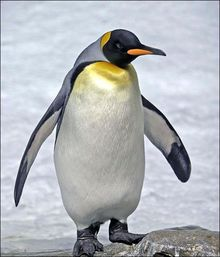
\includegraphics[width = .5\textwidth]{pingouin.jpg}<1>  
  \begin{columns}[t]
      \column{.5\textwidth}
         \only<1>{
           \begin{center}
           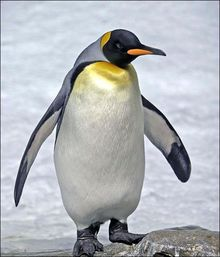
\includegraphics[width = \textwidth]{pingouin.jpg}\\
           Le pingouin de base \ldots
           \end{center}
         }  
         \only<2->{
           \begin{center}
           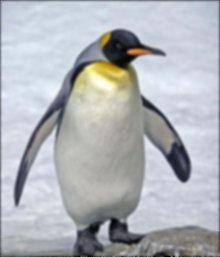
\includegraphics[width = \textwidth]{pingouin2.jpg}\\
           Le pingouin flou \ldots
           \end{center}
         }  
      \column{.5\textwidth}
        \begin{block}{La glisse}
          \begin{itemize}
          \item Il glisse toujours,          
          \item Parfois sur la glace,          
          \item Ou sur la route.
          \end{itemize}
       \end{block}
  \end{columns}
\end{frame}


\end{document}